\subsection{Tensor}
Dalam matematika, tensor didefinisikan sebagai objek geometris yang memetakan himpunan vektor dan kovektor ke dalam sebuah skalar secara linier. Dalam konteks \textit{Deep Learning} dan pengolahan data, tensor lebih sering dipahami sebagai generalisasi dari matriks ke dimensi yang lebih tinggi. Tensor adalah struktur data array multidimensi yang berfungsi sebagai wadah penampung data numerik. Karakteristik utama sebuah tensor ditentukan oleh \textit{Rank} (atau Orde) dan Bentuk/Dimensi-nya.
Secara hierarkis, struktur data dapat diklasifikasikan sebagai tensor dengan rank tertentu:
\begin{IEEEitemize}
    \item Tensor Rank-0 (Skalar) merupakan nilai tunggal (bilangan real). 
        Skalar hanya memiliki besaran (magnitudo) tanpa arah. Notasi matematikanya dapat dituliskan sebagai $x \in \mathbb{R}$.
    \item Tensor Rank-1 (Vektor) merupakan susunan bilangan dalam satu dimensi (\textit{Array 1D}). Vektor memiliki besaran dan arah dalam ruang. 
        Vektor di ruang Euclidean $\mathbb{R}^n$ dinyatakan sebagai $n$-tupel bilangan riil. Dalam matematika, ini dapat dinotasikan sebagai: $\mathbf{v} \in \mathbb{R}^n$
    \item Tensor Rank-2 (Matriks) merupakan susunan bilangan dalam dua dimensi (\textit{Array 2D}) yang terdiri dari baris dan kolom. Matriks merepresentasikan transformasi linier antar ruang vektor. 
        Matriks berukuran $m \times n$ adalah tensor rank-2 dengan bentuk $(m, n)$. Tensor rank-2 dapat dinotasikan sebagai berikut: $A \in \mathbb{R}^{m\times n}$

    \item Tensor Rank-3 dan seterusnya, merupakan susunan bilangan dalam tiga dimensi atau lebih. 
        Tensor rank-3 sering dibayangkan sebagai kubus angka atau tumpukan beberapa matriks. 
\end{IEEEitemize}

Tensor biasanya dinotasikan dengan huruf kapital kaligrafi, misalnya $\mathcal{X}, \mathcal{Y}, \mathcal{Z}$.
Elemen individu dari sebuah tensor dapat diakses menggunakan indeks yang sesuai dengan jumlah dimensinya.
Misalkan $\mathcal{T}$ adalah sebuah tensor rank-3, maka elemen pada posisi $(i, j, k)$ dapat dinotasikan sebagai
$\mathcal{T}_{(i, j, k)}$

Visualisasi dari Tensor Rank-0 sampai Rank-3 dapat dilihat pada Gambar \ref{fig:contoh-tensor} berikut.
\begin{figure}[h]
    \centering
    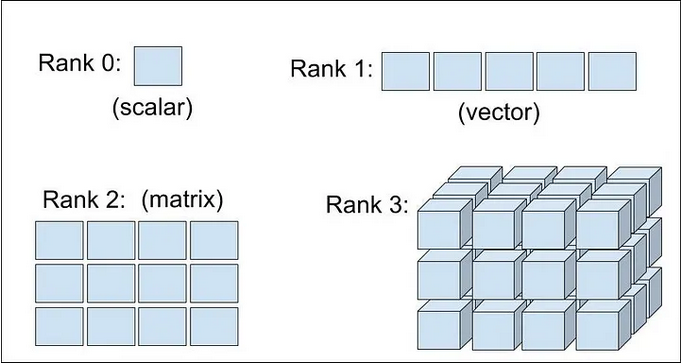
\includegraphics[width=0.4\textwidth]{assets/hierarki-tensor.png}
    \caption{\href{https://thefaheemkhan.medium.com/what-is-tensors-in-machine-learning-4cbf90490a7b}{Visualisasi Tensor Rank-0 sampai Rank-3}}
    \label{fig:contoh-tensor}
\end{figure}

\subsection{Representasi Citra Digital}
Citra digital merupakan representasi diskrit dari suatu gambar kontinu yang telah disampel dalam bentuk grid dua dimensi yang tersusun atas elemen-elemen terkecil yang disebut pixel. Setiap pixel menyimpan informasi intensitas yang umumnya dinyatakan sebagai bilangan bulat, biasanya dapat berupa $[0, 255]$ atau $[0, 1]$ tergantung format penyimpanan dan pemrosesan.
Pada citra \textit{grayscale}, setiap pixel hanya memiliki satu intensitas yang menggambarkan tingkat kecerahan pada posisi tertentu.
Pada citra berwarna, khususnya pada format RGB (\textit{Red, Green, Blue} direpresentasikan oleh tiga komponen intensitas, masing-masing untuk kanal merah, hijau, dan biru. Ketiga nilai ini kemudian dikombinasikan untuk menghasilkan warna akhir pada pixel tersebut.

Secara umum pixel pada citra berwarna dapat dituliskan sebagai
$$
\begin {pmatrix}
    I_{R}(h, w) \\
    I_{G}(h,w) \\ 
    I_{B}(h,w)
\end{pmatrix}
$$

di mana \(I_R(h,w)\), \(I_G(h,w)\), dan \(I_B(h,w)\) menyatakan intensitas kanal merah, hijau, dan biru pada koordinat spasial \((h,w)\).

Pada citra skala keabuan (grayscale), informasi warna diabaikan, dan hanya intensitas cahaya yang disimpan. Citra ini direpresentasikan sebagai matriks.
$$
I \in \mathbb{R}^{H \times W}
$$

Setiap elemen matriks $I_{ij}$ menyimpan nilai skalar yang merepresentasikan kecerahan.

$$
I = \begin{bmatrix}
p_{11} & p_{12} & \cdots & p_{1W} \\
p_{21} & p_{22} & \cdots & p_{2W} \\ 
\vdots & \vdots & \ddots & \vdots \\
p_{H1} & p_{H2} & \cdots & p_{HW}
\end{bmatrix}
$$

Umumnya, nilai $p_{ij}$ dikuantisasi menjadi bilangan bulat dalam rentang $[0,255]$ untuk citra 8-bit, di mana nilai 0 merepresentasikan hitam sempurna dan 255 merepresentasikan putih sempurna.

Pada citra berwarna, umumnya tiap piksel dalam gambar tersusun atas tiga komponen warna dasar, yaitu merah (\textit{red}), hijau (\textit{green}), dan biru (\textit{blue}) atau yang biasa disingkat RGB. 
Sama seperti pada representasi citra \textit{greyscale}, setiap komponen tersebut dapat direpresentasikan dalam rentang nilai 0 hingga 255.
Namun, citra berwarna tidak cukup direpresentasikan oleh satu matriks. Citra berwarna berukuran $H \times W$ direpresentasikan sebagai Tensor Orde-3.
$$
I \in \mathbb{R}^{H \times W \times 3}
$$ 

Setiap piksel pada posisi $(i, j)$ bukan lagi sebuah skalar, melainkan sebuah vektor $\textbf{v} \in \mathbb{R}^{3}$.

$$
\mathbf{v}_{H, W} = 
\begin{pmatrix}
r_{(HW)} \\
g_{(HW)} \\
b_{(HW)} 
\end{pmatrix}
$$

Di mana  $r, g, b$ adalah intensitas masing-masing kanal warna. Dengan demikian nilai $I(h, w, c)$ menyatakan intensitas kanal ke-$c$ pada posisi $(h, w)$ dengan $c$ menyatakan kanal warna (misalnya, R, G, dan B).

Lebih umum, citra dengan \(C\) kanal (misalnya RGB, RGBA, atau representasi fitur lain) dapat ditulis sebagai tensor rank‑3.
$$
I \in \mathbb{R}^{H \times W \times C}.
$$
